\documentclass{standalone}
\usepackage{tikz}
\usetikzlibrary{arrows.meta, positioning, shapes.geometric}

\begin{document}
	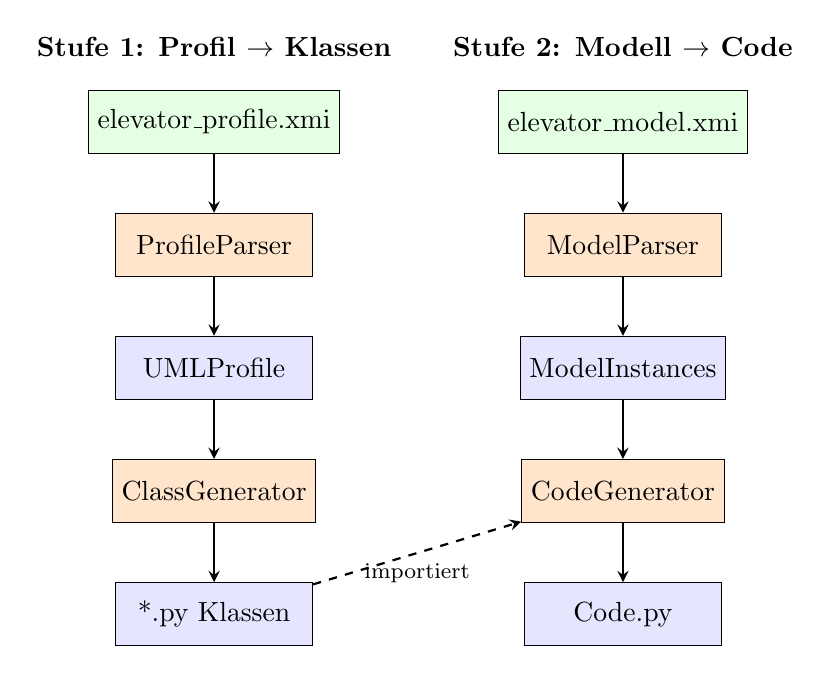
\begin{tikzpicture}[
		node distance=0.75cm and 2cm,
		file/.style={rectangle, draw, fill=green!10, minimum width=2.5cm, minimum height=0.8cm},
		process/.style={rectangle, draw, fill=orange!20, minimum width=2.5cm, minimum height=0.8cm},
		output/.style={rectangle, draw, fill=blue!10, minimum width=2.5cm, minimum height=0.8cm},
		arrow/.style={->, >=stealth, thick}
		]
		\node[file] (profile) {elevator\_profile.xmi};
		\node[process, below=of profile] (parse1) {ProfileParser};
		\node[output, below=of parse1] (umlprofile) {UMLProfile};
		\node[process, below=of umlprofile] (gen1) {ClassGenerator};
		\node[output, below=of gen1] (classes) {*.py Klassen};
		
		\node[file, right=of profile] (model) {elevator\_model.xmi};
		\node[process, below=of model] (parse2) {ModelParser};
		\node[output, below=of parse2] (instances) {ModelInstances};
		\node[process, below=of instances] (gen2) {CodeGenerator};
		\node[output, below=of gen2] (code) {Code.py};
		
		\draw[arrow] (profile) -- (parse1);
		\draw[arrow] (parse1) -- (umlprofile);
		\draw[arrow] (umlprofile) -- (gen1);
		\draw[arrow] (gen1) -- (classes);
		
		\draw[arrow] (model) -- (parse2);
		\draw[arrow] (parse2) -- (instances);
		\draw[arrow] (instances) -- (gen2);
		\draw[arrow] (gen2) -- (code);
		
		\draw[arrow, dashed] (classes) -- (gen2) node[midway, below, font=\footnotesize] {importiert};
		
		\node[above=0.3cm of profile, font=\bfseries] {Stufe 1: Profil $\rightarrow$ Klassen};
		\node[above=0.3cm of model, font=\bfseries] {Stufe 2: Modell $\rightarrow$ Code};
	\end{tikzpicture}
\end{document}